\chapter{Eredmények}
A megtervezett műszaki alkotások értékelése, kritikai elemzése, továbbfejlesztési lehetőségek. 

\section{Képek}
\paragraph{}Itt szerepeljen most pár kép példaként, hogy hogyan lehet őket beszúrni. Fontos, hogy a \LaTeX\ leegyszerűsíti a dolgodat azzal, hogy kitalálja, hogy hova fér el a kép, cserébe nincs abba kifejezetten sok beleszólásod, hogy pontosan hova kerüljön a kép. Ha fontos neked, hogy megmondd, hogy pontosan hol legyen a kép, akkor Google a barátod... Az is fontos, hogy a szövegben minden képre és táblázatra hivatkozz. Például a ~\ref{fig:cat}. ábra egy cicás képet mutat. A szövegben leírtak láthatóak \az ~\ref{fig:rat}. ábrán, illetve \az~\ref{fig:dog1}. és \ref{fig:dog2}.~ábrákon.


\begin{figure}
  \centering
  
\includegraphics[width=0.6\textwidth]{rat}
  \caption{Random kép egy patkányról. A kép szélessége a lap szélességének 0.6-szorosa. Kép forrása: http://www.mmbcc.org.au~\cite{noauthor_ratification}.}
  \label{fig:rat}
\end{figure}

\begin{figure}
  \centering
  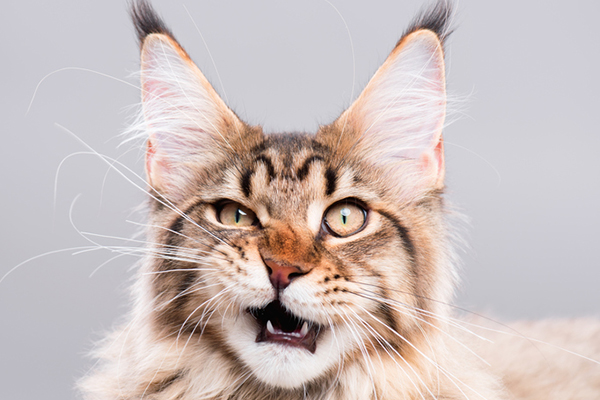
\includegraphics[width=\textwidth]{cat}
  \caption{Random kép egy macskáról. A kép szélessége megegyezik a lap szélességével. Kép forrása: www.theodysseyonline.com~\cite{noauthor_20_2017}.}
  \label{fig:cat}
\end{figure}

\begin{figure}
    \begin{minipage}[c]{0.45\linewidth}
        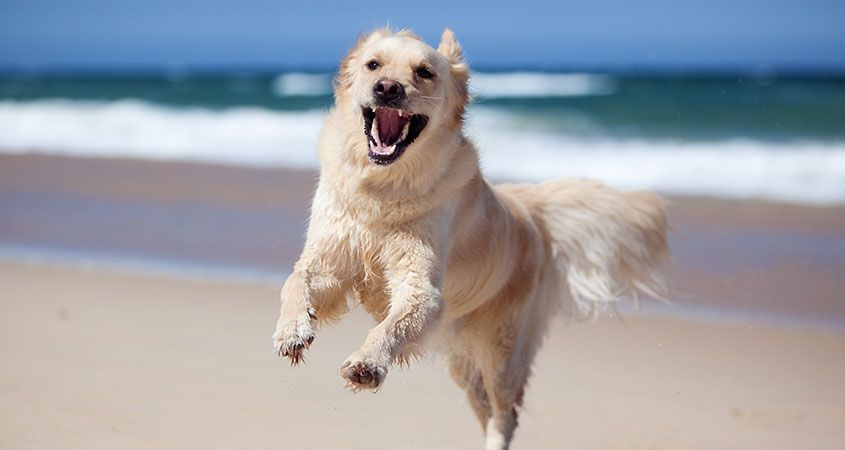
\includegraphics[width=\linewidth]{dog1}
        \caption{Random kép egy kutyáról egy másik kutyás kép bal oldalán. Kép forrása: www.huffingtonpost.ca~\cite{noauthor_get_2016}.}
        \label{fig:dog1}
    \end{minipage}
    \hfill
    \begin{minipage}[c]{0.45\linewidth}
        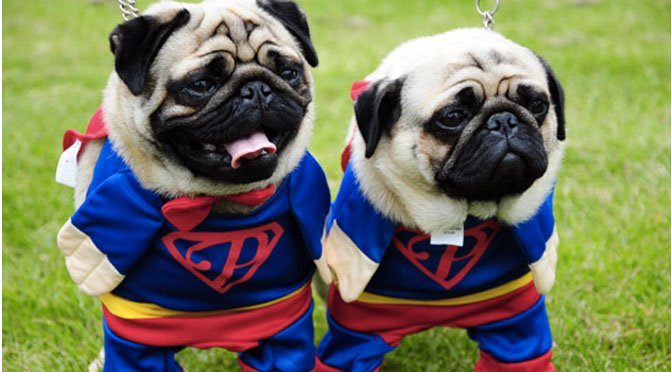
\includegraphics[width=\linewidth]{dog2}
        \caption{Random kép egy kutyáról egy másik kutyás kép jobb oldalán. Kép forrása: imgur.com~\cite{imgur_superman_nodate}.}
        \label{fig:dog2}
    \end{minipage}
\end{figure}

\section{Táblázat}
\paragraph{}Legyen akkor már példa táblázat beillesztésére is. Az \ref{tab:features}.~táblázat a saját szakdogám egy random részéről került beillesztésre.


\begin{table}
\centering
\begin{tabular}{|l|l|l|}
\hline
\rowcolor[HTML]{C0C0C0} 
Positive for... & Negative for... & Number of features \\ \hline
AF & other & 37 \\ \hline
other & normal & 25 \\ \hline
other & AF & 11 \\ \hline
normal & AF & 11 \\ \hline
AF & normal & 1 \\ \hline
\end{tabular}
\caption{Random táblázat.}
\label{tab:features}
\end{table}

\clearpage % új oldalt kezd. A \newline hasonló parancs, de a \clearpage gondoskodik arról, hogy a fentebb beszúrt képek és táblázatok, az alábbi kódok előtt szerepeljenek mindenképp.

\section{Hivatkozás}
Legyen most itt egy hivatkozás Thompson cikkére~\cite{thompson_kennedy_1996}, aminek az adatai a hivatkozasok.bib fájlban található. A hivatkozasok.bib fájlt egyébként érdemes a következő oldal segítségével legenerálni: \url{http://www.citethisforme.com/ieee}. A "More" menü alatt található az "Export" almenüben az "Export as BibTeX" parancs, amivel le lehet tölteni a megfelelő formátumban. Másik opció a zotero használata, ami talán még egyszerűbb, cserébe telepíteni kell: \url{https://www.zotero.org/support/getting_stuff_into_your_library}.

\section{Szövegformázás}
\paragraph{}
\textbf{Legyen itt egy mondat vastagon szedetten.
Meg egy másik, ami \underline{aláhúzásra} is példa + \textit{dőlt betű példa is}.} Utána pedig egy hosszabb térköz.

\vspace{1.5cm}

\section{Forráskód}
Legyen itt egy kis forráskód is:
\lstset{language=Pascal,caption={A Pascal kódrészlet képaláírása.}}
\begin{lstlisting}
for i:=maxint to 0 do
begin
{ do nothing }
end;
Write('Case insensitive ');
Write('Pascal keywords.');
\end{lstlisting}

Meg egy másik, ami teljes fájlt mutat meg, és kódszínezést is mutat:
\lstset{
    language=Python,
    caption={A Python kódrészlet képaláírása.},
    keywordstyle=\color{red},
    stringstyle=\color{blue},
    commentstyle=\color{green},
    morecomment=[l][\color{magenta}]{\#}
}
\lstinputlisting{contents/z_example.py}

\section{Felsorolás}
Végül mutatok egy felsorolást is:
\begin{enumerate}
    \item Első elem
    \begin{itemize}
        \item Valami
        \item Megint valami
        \item Meg valami más
    \end{itemize}
    \item Második elem
    \begin{itemize}
        \item asdf
        \item qwertz
        \item yxcv
    \end{itemize}
    \item Harmadik elem
    \begin{itemize}
        \item Itt a vége
    \end{itemize}
\end{enumerate}

\section{Egyenletek}
És akkor már csak az egyenletek vannak hátra. Itt van egy olyan egyenlet, ami nem kezd új sort: $a^2 + b^2 = c^2$ vagy $\sum_{i = 0}^{n}a_i - \int_{0}^{\pi}f(x)dx$. De van olyan is, ami új sort kezd (két dollár-jellel kezdem és fejezem be): $$\frac{-b\pm\sqrt{b^2-4ac}}{2a}.$$
Ha pedig arra van szükségem, hogy számozott legyen az egyenlet, és pl hivatkozni tudjak a \ref{eq:bonyolult}.~egyenletre, akkor így lehet csinálni:
\begin{equation} \label{eq:bonyolult}
    \sum_{i=1}^{\left[\frac{n}{2}\right]}\binom{x_{i,i+1}^{i^{2}}}
    {\left[\frac{i+3}{3}\right]}\frac{\sqrt{\mu(i)^{\frac{3}{2}}(i^{2}-1)}}{\sqrt[3]{\rho(i)-2}+\sqrt[3]{\rho(i)-1}}
\end{equation}

Egyenletek \LaTeX kódjának írását hamar elsajátíthatja az ember némi googlizás árán, viszont van erre online szerkesztő is: \url{http://www.hostmath.com/}.

\newpage

\section{Hosszú idézet}
\paragraph{Random szöveg az idézet előtt.}\lipsum[2]
\begin{displayquote}
    The 2017 PhysioNet/CinC Challenge aims to encourage the development of algorithms to classify, from a single short ECG lead recording (between 30 s and 60 s in length), whether the recording shows normal sinus rhythm, atrial fibrillation (AF), an alternative rhythm, or is too noisy to be classified.
    
    Previous studies concerning AF classification are generally limited in applicability because 1) only classification of normal and AF rhythms were performed, 2) good performance was only shown on carefully-selected often clean data, 3) a separate out of sample test dataset was not used, or 4) only a small number of patients were used. 
    It is challenging to reliably detect AF from a single short lead of ECG, and the broad taxonomy of rhythms makes this particularly difficult. 
    In particular, many non-AF rhythms exhibit irregular RR intervals that may be similar to AF. 
    In this Challenge, we treat all non-AF abnormal rhythms as a single class and require the Challenge entrant to classify the rhythms as 1) Normal sinus rhythm, 2) AF, 3) Other rhythm, or 4) Too noisy to classify.
\end{displayquote}
\begin{flushright}-------------- Introduction to \textit{Computing in Cardiology Challenge of 2017}\end{flushright}

\paragraph{Random szöveg az idézet után.}\lipsum[2]

\clearpage % Ez azért kell, hogy nehogy képek átcsússzanak a következő fejezethez